
\iffalse
\begin{figure}
    \centering
    \includegraphics[width=12cm]{../figures/blip_bbh_runs_two_panel_comparison.pdf}
    \caption{Glitch panel comparison}
    \label{fig:qscan_null}
\end{figure}
\fi
While the third-generation detectors are anticipated to push the accuracy and precision of our measurements to unprecedented levels, they will also be subject to new kinds of challenges compared to the current generation detectors. Here, I specifically compare the problem posed by glitches to the LIGO-Virgo interferometers and third-generation interferometers. 
\begin{table}[h!]
    \centering
    \renewcommand{\arraystretch}{1.2}
    \begin{tabular}{p{0.45\textwidth}|p{0.45\textwidth}}
    \toprule
    \textbf{LIGO-Virgo interferometers} & \textbf{Third-generation interferometers} \\
    \midrule
    \begin{enumerate}[leftmargin=*, label=\arabic*.]
        \item Detection rate of $\mathcal{O}(1)$ signal per week
        \item A GW signal is in-band for $\mathcal{O}(1)$ second to $\mathcal{O}(1)$ minute. Therefore, nearly every segment of data contains only noise. 
        \item Glitch rate of $\mathcal{O}(1)$ per minute across three observation runs. 
        \item \textit{Almost} all glitches occur in isolation due to a smaller in-band duration and smaller detection rate of GW signals. 
        \item Almost all glitches can be vetoed without incurring a significant loss of GW signals. 
    \end{enumerate}
    &
    \begin{enumerate}[leftmargin=*, label=\arabic*.]
        \item Detection rate of $\mathcal{O}(1)$ signal per minute
        \item A GW signal is in-band for $\mathcal{O}(1)$ minute to $\mathcal{O}(1)$ hour. Therefore, nearly every segment of data is expected to contain a signal. 
        \item Glitch rate is unknown. Let's assume the same as LIGO-Virgo interferometers.
        \item \textit{Almost} all glitches will overlap with a GW signal due to a larger in-band duration and larger detection rate. 
        \item Very few glitches may be vetoed without losing GW signals. 
    \end{enumerate}
    \\
    \bottomrule
    \end{tabular}
    \caption{Problem posed by glitches in LIGO-Virgo interferometers versus third-generation interferometers.}
    \label{tab:glitch_diff}
\end{table}
When occurring in the vicinity of a GW signal, glitches (or transient noises) can corrupt the signal. Such signal-overlapping glitches must be carefully removed before analysing the signal. From the 90 confident events detected across three observation runs by LIGO-Virgo interferometers, about 20 were contaminated by glitches and required some form of glitch mitigation~\cite{KAGRA:2021vkt}. This number will continue to increase as the interferometers collect more data. A detailed study on how the physical interpretation of a GW signal may vary, depending on how a glitch in its proximity is removed, was conducted in the context of GW191109~\cite{Udall:2024ovp}. Specifically, it was argued that the interpretation of the spins of black holes may be affected. 

While glitch mitigation is an active area of research for current generation detectors, it is yet to receive similar attention in the context of 3G detectors. In Table~\ref{tab:glitch_diff}, we compare the problem posed by glitches for the LIGO-Virgo and the 3G interferometers. Glitches could be a major bottleneck in transitioning to the precision science era. In this chapter, we introduce the \texttt{nijntje} -- a null stream inspired noise transient elimination framework that is inexpensive, accurate, and scalable against the increasing computational cost of data analysis in the 3G-era. Through \texttt{nijntje}, we demonstrate a clear edge that the null stream inherent in the triangular configuration of the Einstein Telescope provides for the precision science era. 


\section{The null stream}
By definition, a null stream is a linear combination of strain data from a network of GW detectors such that the signal (if present in the strain) cancels out. For the triangular configuration of the Einstein Telescope (\ETT), the null stream can be constructed by summing the strain data from three interferometers. Let us denote the data from $i^{\mathrm{th}}$ interferometer by $\vec{d}_i$,
\begin{equation}
 \vec{d}_i = F_{+, i} \vec{h}_+ + F_{\times, i} \vec{h}_{\times},
\end{equation}
where $i$ varies from 1 to 3, $F_+$ and $F_{\times}$ are the antenna pattern functions, $h_+$ and $h_{\times}$ are the GW polarizations, defined in chapter~\ref{ch:gws}. The null stream is then given by
\begin{equation}
    \label{eq:null-stream-eq}
 \vec{d}_{\mathrm{null}} = \frac{1}{\sqrt{3}}\sum_{i = 1}^{3}\vec{d}_i,
\end{equation}
where the prefactor of $1/\sqrt{3}$ ensures that the noise’s power spectral density of the null stream equals the average of those of the individual detectors. 

\begin{figure}
    \centering
    \includegraphics[width=\textwidth]{../figures/null_stream_antenna_pattern.pdf}
    \caption{Illustration of how the null stream of \ETT~comes about. Projection of plus (left) and cross (right) antenna pattern functions along the right ascension (RA) coordinate. Blue, red, and green lines show the antenna pattern functions of ET$_1$, ET$_2$, and ET$_3$, respectively. The black line, which is equal to zero for all values of RA, is obtained by summing the three. This feature gives rise to an inherent null stream in the triangular configuration of ET.}
    \label{fig:sum_patterns}
\end{figure}

The null stream is a geometric feature of the triangle configuration of ET. It comes about from the fact that the sum of antenna pattern functions is individually zero \asam{Somewhere maybe the expressions for F+ and Fx; or you could put it in chapter 1 just after Eqn (1.33) and refer to it here as well.}, i.e.,
\begin{equation}
    \label{eq:sum_pattern}
    \sum_{i=1}^3 F_{+, i} = 0 ~ ~ \mathrm{and} ~ ~ \sum_{i=1}^3 F_{\times, i} = 0.
\end{equation}
Indeed, the individual antenna pattern functions vary over the whole sky and the equalities presented in Eq.~\eqref{eq:sum_pattern} hold for the whole sky as well. As an illustration, we show the projection of antenna pattern functions along the right ascension (RA) coordinate.


\section{\texttt{nijntje}: null-stream inspired noise transient elimination framework}
\label{sec:framework}
The null stream of the triangular ET enables a novel framework to remove signal-overlapping glitches. For brevity, we refer to it as \texttt{nijntje} -- null-stream inspired noise transient elimination -- framework. Figure~\ref{fig:nijntje_chart} shows the workflow of the \texttt{nijntje} framework.
\begin{figure}
    \centering
    \includegraphics[width=16cm]{../figures/assemble_nijntje.pdf}
    \caption{The blue box outlines the workflow of \texttt{nijntje} framework. \textit{Step 1}: Construct the null stream by summing the strain data from three interferometers. \textit{Step 2}: Using the null stream data and an RJMCMC method, perform an unmodelled reconstruction of the glitch timeseries. \textit{Step 3}: Subtract the glitch timeseries from $\mathrm{ET}_1$ frame to obtain the \textit{cleaned} frame. \textit{Step 4} (Optional): Perform parameter estimation of the GW signal using the cleaned data from $\mathrm{ET}_1$, and the existing data from $\mathrm{ET}_2$ and $\mathrm{ET}_3$ to verify the accuracy of glitch mitigation.}
    \label{fig:nijntje_chart}
\end{figure}
\subsubsection{Setup of the simulation}
We consider a typical scenario where a glitch overlaps with a GW signal. While the glitches exhibit a range of morphology, here we choose a morphology that is ubiquitous in the data, i.e. the blips. For the sake of the example, we assume that the only interferometer encounters the glitch. The rest of the two interferometers of the triangle contain a GW signal in Gaussian noise. The GW source is placed at a redshift of 2, where the merger rate distribution of BBH peaks, making it a typical source. The source frame masses of the two black holes are $38\,M_\odot$ and $33\,M_\odot$. This choice of parameters results in a GW signal with a network signal-to-noise ratio (SNR) of 83 divided equally among three interferometers. The starting frequency of our analysis is 20 Hz, the sampling frequency is 2048 Hz, and we use ET-D PSD to simulate Gaussian noise. We inject a blip glitch in the ET$_1$ interferometer that overlaps with the GW signal. We ensure that the SNR of the glitch is similar to the SNR of the GW signal in ET$_1$, i.e. $83/\sqrt{3} \sim 47$. Thanks to recent developments in machine learning based methods, it is now possible to simulate glitches.  
For example, the \texttt{gengli} codebase can generate blip glitches akin to the ones observed during the second observing run of Advanced LIGO and Virgo~\cite{Lopez:2022lkd, Lopez:2022dho}. An illustration of this setup is shown in the top panel of Figure~\ref{fig:nijntje_chart}. 

\subsubsection{Executing the steps of \texttt{nijntje} framwork}
Following the steps outlined in Figure~\ref{fig:nijntje_chart}, we first formulate the null stream. By construction, the null stream does not contain any signal. It only contains the glitch and the sum of Gaussian noise from three interferometers. In order to subtract the glitch, we first need to reconstruct the corresponding timeseries. We do this using the unmodelled reconstruction method described in chapter \ref{ch:bayeswave}. Indeed, we do not need to be concerned about the possible leakage from the GW signal while performing the glitch reconstruction using the null stream. Once the glitch is reconstructed from the null stream, we obtain the timeseries corresponding to the median parameters of the posterior samples and subtract it from the ET$_1$ frame file. This completes our step 3 and provides us with the \textit{cleaned} GW signal. Next, to verify that our glitch mitigation is accurate, i.e., we have not removed part of the signal or we have not left behind a part of the glitch, we perform modelled reconstruction (also known as parameter estimation) on the GW signal, as described in chapter~\ref{ch:gwpe}. 


\section{Glitch mitigation in the absence of \texttt{nijntje} framework}
The framework \texttt{ninjtje} is unique to the triangular geometry of the ET. To compare \ETT~with an alternate configuration, we consider a network of two, distant L-shaped interferometers (referred to as ET-2L) located in Sardinia and the EMR region. In the absence of \texttt{nijntje} framework, we perform a joint reconstruction of the GW signal and the glitch using the data from both interferometers. The joint modelling is prone to leakage, i.e, part of the glitch could be mismodelled as a signal and vice versa. Therefore, as introduced in Chatziioannou \textit{et al.}~\cite{Chatziioannou:2021ezd}, instead of modelling the GW signal itself with sine-Gaussian wavelets, a realistic signal model is employed with the expectation of reducing the mismodelling.

The setup of the simulation for the ET-2L network remains similar to the one described in section~\ref{sec:framework}. The GW signal parameters and the glitch morphology are the same as triangular ET, leading to a GW network SNR 
of 124, with the Sardinia and EMR interferometers contributing SNRs of 90 and 85, respectively. The glitch is introduced in the Sardinia interferometer, the SNR of which matches the glitch SNR in ${\rm ET}_1$. For this setup, we perform a glitch mitigation using the BayesWave codebase -- a routinely used tool to perform joint modelling of the GW signal and glitch coherently across the detector network. To reiterate, the GW signal here is modelled using the signal model, i.e. the IMRPhenomD model, and the glitch is modelled using wavelets. While one can model both the signal and the glitch, using wavelets, this approach increases the amount of mismodelling and is hence not preferred. 

\begin{figure}[h]
    \centering
    \includegraphics[width=.4\textwidth]{../figures/thesis_et2l_delta_glitch_overlap_glitch_master.pdf}\hspace{.5cm}
    \includegraphics[width=.4\textwidth]{../figures/thesis_newsnr_mismatch_comparison.pdf}
    \caption{Green (red) indicates the glitch reconstructed using \ETT~null stream (ET-2L) for the $\Delta t = 0$ case. Grey shows the strain, and black shows the simulated glitch. The null stream helps avoid glitch mismodeling, resulting in much closer agreement with the simulated glitch.}
    \label{fig:glitch_overlap}
\end{figure}

\section{Results of source parameter measurement: Triangle and 2L comparison}

For each configuration, \ETT and 2L, we consider 9 different scenarios. All settings are kept identical across these scenarios except the time interval between the GW merger and glitch onset. For \ETT, we perform glitch mitigation using \texttt{nijntje} and obtain cleaned frames. For ET-2L, in the absence of \texttt{nijntje} framework, we perform glitch mitigation by doing joint signal plus glitch modelling. After the glitch is removed, we perform the parameter estimation to quantify the accuracy of glitch mitigation. If the glitch mitigation is precise, the measurement should be similar to a scenario where a glitch is not introduced to the data. 

Before we present the parameter estimation results, we showcase the results of glitch mitigation, i.e., how close the reconstructed glitch is to the true glitch. This serves as a precursor to the parameter estimation results since accurate glitch mitigation leads to accurate parameter measurement. A visualisation of the glitch reconstruction is presented in Figure~\ref{fig:glitch_overlap}. The ET triangle configuration, due to the null stream, achieves a more accurate glitch reconstruction by avoiding mismodeling from the GW signal. In contrast, for the ET-2L configuration, inevitably, some additional features from the signal are incurred. 

\begin{figure}[h]
    \centering
    \includegraphics[width=\textwidth]{../figures/newsnr_fig_4.pdf}
    \caption{Measurement of detector-frame total mass $M_{\rm total}$, luminosity distance $D_{\rm L}$, 
 and sky localization. Green (red) colour represents posterior distributions when the glitch is 
 removed using the \ETT~null stream (ET-2L). Blue colour shows the measurements when no glitch is 
 introduced, serving as a benchmark for comparison, and dashed black lines indicate the true values. 
 The green posteriors accurately recover the true parameter values and show high consistency 
 with the benchmark. Though the red posterior for the total mass $M_{\rm total}$ recovers the true value, it shows clear signs of bias and widening. In contrast, the measurements of luminosity distance and sky location are biased and miss the true values.}
    \label{fig:delta_zero}
\end{figure}


\iffalse
\begin{figure}
    \centering
    \includegraphics[width=10cm]{../figures/newsnr_mismatch_comparison.pdf}
    \caption{Mismatch}
    \label{fig:mismatch}
\end{figure}
\fi
\subsubsection{Glitch onset coinciding with the GW merger}

Next, we turn to the results of parameter estimation when the glitch precisely coincides with the GW merger. Figure~\ref{fig:delta_zero} presents a comparison of the posterior distributions of the GW signal parameters after the glitch is mitigated, for $\Delta t = 0$. For all parameters shown, glitch mitigation with null stream for \ETT~results in posteriors 
that demonstrate high consistency and closely align with the benchmark results, where ``benchmark'' refers to a scenario when no glitch is introduced to the data.

For the ET-2L configuration, though the total mass $M_{\rm total}$ posterior shows clear signs of widening, it recovers the true value. This can be attributed to the SNR 
in the glitch-free interferometer, enabling intrinsic parameter recovery. In contrast, posteriors for extrinsic parameters, 
namely luminosity distance and sky location, are inconsistent with the benchmark's posteriors and miss the true value. 

\begin{figure}[h]
    \centering
    \includegraphics[width=.45\textwidth]{../figures/newsnr_rank_10_single_block_percentile_parameters_short.pdf}
    \caption{A comparison of the credible level of the true parameter value relative to the posterior 
 distributions for various time intervals $\Delta t$ between glitch onset and GW merger. 
 Credible levels are in standard deviation units $\sigma$, following a standard normal distribution. The parameters considered are luminosity distance $D_{\rm L}$ and sky location $\Omega$. Green (red) markers denote credible levels for the \ETT~null stream (ET-2L) based measurements, and the blue lines provide credible levels in the absence of a 
 glitch as a benchmark (dotted for $\Omega$, dashed for $D_{\rm L}$). For the null stream-based approach, the credible levels closely align with the benchmark, indicating accurate measurements. The posteriors for ET-2L lead to wider credible levels and generally exclude the true value, except for the edge cases where the glitch is sufficiently distant in time from the GW merger.}
    \label{fig:trend}
\end{figure}

\subsubsection{Glitch onset away from the GW merger}

Finally, we turn to the scenarios when the glitch does not coincide with the merger. Figure~\ref{fig:trend} shows that the characteristics of extrinsic parameter recovery remain consistent 
across different $\Delta t$ values. A negative (positive) value of $\Delta t$ implies that the glitch 
onset falls before (after) the GW merger. For all time intervals considered, the~\ETT~configuration 
yields measurements where the true distance and sky location lie within $3\sigma$ and closely 
align with the no-glitch benchmark. In contrast, with the ET-2L configuration, the resulting measurements 
are wider or generally exclude the true values, except when the glitch onset is 100 ms before or 20 ms after the merger. We infer that at those values of $\Delta t$, the glitch is far enough from the GW signal to cause any biases. 


\section{Conclusions and future work}
The null stream provides us with an extra piece of information in the form of Eq.~\eqref{eq:null-stream-eq}. For the first time, we quantitatively show how this information can be used to address the problem posed by glitches. Further, in the table \ref{tab:nijntje_conclusion}, we present a qualitative comparison between the \ETT and ET-2L~configuration in the context of glitch mitigation. 

\begin{table}[h!]
    \centering
    \renewcommand{\arraystretch}{1.2}
    \begin{tabular}{p{0.45\textwidth}|p{0.45\textwidth}}
    \toprule
 Glitch mitigation using ET-2L & Glitch mitigation using \ETT \\
    \midrule
    \begin{enumerate}[leftmargin=*, label=\arabic*.]
        \item Biases expected in the measurements.
        \item True signal model needs to be known \textit{a priori}. Biases worsen if the signal model is not known or incorrect.
        \item $\mathcal{O}(10)$ hours per analysis. Difficult to scale to meet the demands of the 3G era. \textcolor{white}{lorem ipsum lorem ipsum.}
        \item Modification required depending on the type of the GW signal and glitch. Modification required when multiple signals and glitches are overlapping with each other -- a scenario highly likely in the 3G era.
        \item Biases worsen when two interferometers have unequal SNRs.
    \end{enumerate}
    &
    \begin{enumerate}[leftmargin=*, label=\arabic*.]
        \item Quality of measurements is identical to the scenario when glitches are not introduced.
        \item Does not require any prior knowledge of the signal model. Ready-to-use for all kinds of signals. 
        \item $\mathcal{O}(1)$ hour per analysis. Fast and accurate framework \texttt{nijntje}; a ready-to-use tool for the triangular ET. 
        \item Ready-to-use against varying morphologies of glitches. Ready-to-use even when multiple signals and glitches are overlapping. \textcolor{white}{lorem ipsum lorem ipsum lorem ipsum dolor lorem ipsum}
        \item Individual interferometer SNRs do not play any role. 
    \end{enumerate}
    \\
    \bottomrule
    \end{tabular}
    \caption{Comparison \ETT~and ET-2L configuration in context of glitch mitigation}
    \label{tab:nijntje_conclusion}
\end{table}

We plan to extend this work by including various kinds of signals and glitches in our analysis. We also plan to investigate the possibility of occurrence and mitigation of coincident glitches, i.e., glitches that appear in all interferometers of a network at the same time. We also plan to investigate the impact of Newtonian noise -- the models of which are poorly known at the time of writing of this thesis. In addition, the null stream can be constructed when all three interferometers are online. We leave it to future work to include the duty cycle in our analysis. Note that, in the absence of a null stream, one can revert to performing joint signal and glitch mitigation for the triangular configuration.

The problem posed by glitches to the current and next-generation GW detectors is a pressing one. It could hinder our transition to the precision science era. The comparison presented in this chapter shows a clear edge that the null stream inherent in the triangular configuration has to offer over the alternate configuration. 

